% Corrigé de l'exercice 13_TransfoMouvement.
% Version autonome : aucune image de correction extérieure n'est nécessaire.
\begin{corrigebox}[Corrigé complété]

\CorrigeQuestion{1}
Le mécanisme comporte quatre solides. La manivelle \textbf{1} est en liaison
pivot avec le bâti \textbf{0} en $A$. La pièce coulissante \textbf{3} est en
liaison pivot avec la manivelle en $B$ et en liaison glissière avec le corps
oscillant \textbf{2}. Ce dernier est en liaison pivot avec le bâti en $C$.
\begin{center}
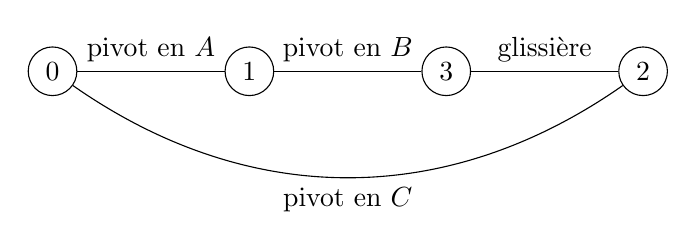
\begin{tikzpicture}[>=latex,node distance=2.5cm]
  \node[draw,circle] (S0) {$0$};
  \node[draw,circle,right of=S0] (S1) {$1$};
  \node[draw,circle,right of=S1] (S3) {$3$};
  \node[draw,circle,right of=S3] (S2) {$2$};
  \draw[-] (S0) -- node[above]{pivot en $A$} (S1);
  \draw[-] (S1) -- node[above]{pivot en $B$} (S3);
  \draw[-] (S3) -- node[above]{glissière} (S2);
  \draw[-] (S2) to[bend left=35] node[below]{pivot en $C$} (S0);
\end{tikzpicture}
\end{center}

On choisit $C$ comme origine, avec $\vect{CA}=H\vect{j_0}$. La position du
point $B$ est alors
\[
\overrightarrow{CB}=R\cos\theta\,\vect{i_0}
 +\left(H+R\sin\theta\right)\vect{j_0}.
\]
La position de la pièce coulissante dans le corps oscillant est donc donnée
par
\[
s(\theta)=CB
=\sqrt{R^2+H^2+2HR\sin\theta}.
\]

\CorrigeQuestion{2}
Pour $\theta=\dfrac{\pi}{2}$, le point $B$ se trouve sur l'axe vertical au-dessus
de $A$ :
\[
B=(0,H+R),\qquad CB=H+R=70\,\mathrm{mm}.
\]
Le corps oscillant est vertical et la pièce \textbf{3} est dans sa position
la plus sortie.

\CorrigeQuestion{3}
Pour $\theta=0$, on obtient
\[
B=(R,H),\qquad CB=\sqrt{R^2+H^2}
=\sqrt{30^2+40^2}=50\,\mathrm{mm}.
\]
L'axe du corps oscillant fait avec la verticale l'angle
\[
\beta=\arctan\!\left(\frac{R}{H}\right)
=\arctan\!\left(\frac{30}{40}\right)\simeq36{,}9^\circ.
\]

\CorrigeQuestion{4}
Pour $\theta=-\dfrac{\pi}{2}$, le point $B$ est situé entre $C$ et $A$ :
\[
B=(0,H-R),\qquad CB=H-R=10\,\mathrm{mm}.
\]
Le corps oscillant est de nouveau vertical et la pièce \textbf{3} est dans
sa position la plus rentrée.

\CorrigeQuestion{5}
La course est la différence entre les positions extrêmes :
\[
\mathcal{C}=s_{\max}-s_{\min}
=(H+R)-(H-R)=2R.
\]
Avec $R=30\,\mathrm{mm}$ :
\[
\boxed{\mathcal{C}=60\,\mathrm{mm}}.
\]

\end{corrigebox}
